\section{Техническое задание}
\subsection{Основание для разработки}

Полное наименование системы: «Программное обеспечение для системы контроля и управления доступом на круизном судне».
Основанием для разработки программы является приказ ректора ЮЗГУ от «15» апреля 2024 г. №1779-с «Об утверждении тем выпускных квалификационных работ».

\subsection{Цель и назначение разработки}

Целью данной работы является проектирование базы данных круизного лайнера и разработка приложения для карт доступа пассажиров.

В настоящее время перед СКУД стоят задачи: четкое и быстрое регулирование правил доступа во время поездки и обеспечение безопасной эвакуации пассажиров в случае ЧС. Для выполнения этих задач требуется систематизация данных. 

Основными задачами при проектировании и разработке базы данных  и приложения являются:
\begin{itemize}
	\item исследование предметной области;
	\item проектирование базы данных;
	\item создание базы данных;
	\item заполнение базы данных информацией;
	\item разработка  интерфейса;
	\item реализация приложения.
\end{itemize}

\subsection{Требования к интерфейсу}

Приложение должно включать в себя:
\begin{itemize}
	\item навигацию по таблицам;
	\item отдельные интерфейсы для каждой таблицы с полями;
	\item отображение текущей таблицы в реальном времени(TreeView);
	\item возможность так или иначе воздействовать на внесённые данные базы внутри приложения;
	\item понятную навигацию и легкий поиск среди элементов конкретной таблицы;
	\item отображение локального времени во избежание ошибок;
\end{itemize}

\subsection{Требования к программной системе приложения <<СКУД на круизном лайнере>>}
\subsubsection{Требования к данным программной системы}

Система должна уметь эффективно обрабатывать данные пассажиров, включая личную информацию, данные о тарифе, информацию о штрафах и спутниках. Необходимо обеспечить конфиденциальность и безопасность этих данных.

Потенциальные объекты:
\begin{itemize}
	\item ДОСТУПЫ;
	\item ДОСТУПЫ-ЧС;
	\item ПАССАЖИРЫ;
	\item ДВЕРИ;
	\item КОМНАТЫ;
	\item ШТРАФЫ;
	\item ДЕТИ;
\end{itemize}


\subsection{Построение ER-модели данных}

На основе анализа неформального описания предметной области были определены наборы объектов и связей.

\subsubsection {Определение объектов}

Потенциальные объекты и атрибуты, включая необязательные:
Пассажир
\begin{itemize}
	\item (Первичный)ID
	\item *Имя
	\item *Фамилия
	\item *Возраст
	\item *Пол
	\item *Тариф
	\item ○Медицинские заметки
	\item ○Судимости
	\item *Комната
	\item ○Образование 
	\item ○Квалификация	
\end{itemize}

Ребёнок
\begin{itemize}
	\item (Первичный)ID
	\item *Имя
	\item *Фамилия
	\item *Возраст
	\item *Пол
	\item *Тариф
	\item *Спутник
	\item ○Медицинские заметки
	\item ○Судимости
	\item *Комната	
\end{itemize}

Дверь
\begin{itemize}
	\item (Первичный)ID
	\item *Наименование
	\item *Комната,в которую ведёт
	\item ○Системное время
	\item ○Номер
	\item *Статус
	\item *Скорость закрытия
	\item ○Ограничитель
\end{itemize}

Комната
\begin{itemize}
	\item (Первичный)ID
	\item *Наименование
	\item *Кол-во дверей
	\item *Тип
	\item ○Ограничение по времени (ближайшее мероприятие)
	\item ○Ограничение по полу
	\item ○Ограничение по медицинской карте
	\item ○Ограничение по судимости
	\item ○Ограничение по штрафу	
\end{itemize}

Штраф
\begin{itemize}
	\item (Первичный)ID
	\item ○Время наложения
	\item *Действителен ли
	\item *Возможно ли снять
	\item ○Сумма выкупа
	\item *Вид
	
\end{itemize}

\subsubsection{Определение связей}

Слева направо: Каждый пассажир (ПАССАЖИР) может сопровождать ребёнка(РЕБЁНОК).

Справа налево: каждый ребёнок(РЕБЁНОК) должен быть сопровождаем Пассажиром(ПАССАЖИР).

Слева направо: Каждый пассажир(ПАССАЖИР) или ребёнок(РЕБЁНОК) имеет свою личную комнату(КОМНАТА).

Справа налево: Каждая жилая комната(КОМНАТА) может принадлежать пассажиру(ПАССАЖИР) или ребёнку(РЕБЁНОК). 

Слева направо: Каждый пассажир(ПАССАЖИР) может иметь штрафы(ШТРАФ).

Справа налево: каждый штраф(ШТРАФ) должен быть закреплён за  пассажиром(ПАССАЖИР)-нарушителем.

Слева направо: каждая дверь(ДВЕРЬ) может вести в комнату(КОМНАТА).

Справа налево: Каждая комната(КОМНАТА) имеет ведущие в неё двери (ДВЕРЬ).

Слева направо: каждый пассажир(ПАССАЖИР) или ребёнок(РЕБЁНОК) имеют доступы к дверям(ДВЕРЬ).

Справа налево: Каждая дверь(ДВЕРЬ) предоставляет доступы пассажирам(ПАССАЖИР) или детям(РЕБЁНОК).

\subsubsection{Определение кардинальности связей}

Слева направо: Каждый пассажир (ПАССАЖИР) может сопровождать одного и более ребёнка(РЕБЁНОК).

Справа налево: каждый ребёнок(РЕБЁНОК) должен быть сопровождаем одним Пассажиром(ПАССАЖИР).

Слева направо: Каждый пассажир(ПАССАЖИР) или ребёнок(РЕБЁНОК) имеет одну личную комнату(КОМНАТА).

Справа налево: Каждая жилая комната(КОМНАТА) может принадлежать одному или многим пассажирам(ПАССАЖИР) или детям(РЕБЁНОК).

Слева направо: Каждый пассажир(ПАССАЖИР) может иметь 1 или несколько штрафов(ШТРАФ).

Справа налево: каждый штраф(ШТРАФ) должен быть закреплён за одним пассажиром(ПАССАЖИР)-нарушителем.

Слева направо: каждая дверь(ДВЕРЬ) может вести в одну комнату(КОМНАТА).

Справа налево: Каждая комната(КОМНАТА) имеет одну или несколько дверей (ДВЕРЬ).

Слева направо: каждый пассажир(ПАССАЖИР) или ребёнок(РЕБЁНОК) имеют доступ к одной или нескольким дверям(ДВЕРЬ).

Справа налево: Каждая дверь(ДВЕРЬ) предоставляет доступы сразу нескольким пассажирам(ПАССАЖИР) или детям(РЕБЁНОК).

\subsubsection{Разрешение связи <<Многие ко многим>>}

Описание решения Связи M:M между объектами ПАССАЖИР и ДВЕРИ, РЕБЁНОК И ДВЕРИ необходимо решить с помощью объектов пересечения. 

Это объекты пересечения с именами ДОСТУПЫ и ДОСТУПЫ ЧС, в которых хранится информация о предоставленном доступе к дверям в обычной и чрезвычайной ситуациях, исходя из сравнения ограничений с обеих сторон. Это дает нам возможность привязывать пассажиров/детей к дверям.
 
Идентификаторы PkID для объектов ДОСТУП/ДОСТУП ЧС использует ассоциативную связь для применения UID из обоих объектов ПАССАЖИР(РЕБЁНОК) и ДВЕРЬ в качестве PkID.

После добавления объектов пересечения появились следующие связи:

Слева направо: Каждый Пассажир(ПАССАЖИР) имеет несколько доступов(ДОСТУП) к дверям и доступов к дверям в случае ЧС (ДОСТУП ЧС).

Справа налево: Каждый Доступ(ДОСТУП) или (ДОСТУП ЧС) предоставляется лишь одному пассажиру(ПАССАЖИР).

Слева направо: Каждый Ребёнок имеет несколько доступов(ДОСТУП) к дверям и доступов к дверям в случае ЧС (ДОСТУП ЧС).

Справа налево: Каждый Доступ(ДОСТУП) или (ДОСТУП ЧС) предоставляется лишь одному ребёнку(РЕБЁНОК).

Слева направо: Каждая дверь(ДВЕРЬ) предоставляет несколько доступов(ДОСТУП)/(ДОСТУП ЧС).

Справа налево: каждый доступ (ДОСТУП)/(ДОСТУП ЧС) запрашивается только от одной двери(ДВЕРЬ)

\subsubsection{Извлечение вторичных ключей из простых объектов с помощью внешних ключей}

Связь 1:М между объектами ПАССАЖИР и ШТРАФ необходимо решить с помощью внешнего ключа. 
Внешний ключ хранится в поле объекта ШТРАФ(Принадлежность) и является обязательным. Это дает нам возможность привязывать каждый штраф к нарушителю.
 
Идентификатор FkID для объекта Штрафы ссылается на UID Пассажира.
Связь 1:М между объектами ПАССАЖИР и РЕБЁНОК необходимо решить с помощью внешнего ключа. 
Внешний ключ хранится в поле объекта РЕБЁНОК(Спутник) и является обязательным. Это дает нам возможность привязывать каждого ребёнка к его сопровождающему.
 
Идентификатор FkID для объекта Ребёнок ссылается на UID Пассажира.
Связь М:1 между объектами ПАССАЖИР и КОМНАТА необходимо решить с помощью внешнего ключа. 
Внешний ключ хранится в поле объекта ПАССАЖИР(Комната) и является обязательным. Это дает нам возможность закреплять каждого пассажира за своей комнатой.
 
Идентификатор FkID для объекта ПАССАЖИР ссылается на поле номера ДВЕРИ, ведущей в эту КОМНАТУ.
Связь М:1 между объектами РЕБЁНОК и КОМНАТА необходимо решить с помощью внешнего ключа. 
Внешний ключ хранится в поле объекта РЕБЁНОК(Комната) и является обязательным. Это дает нам возможность закреплять каждого пассажира за своей комнатой.
 
Идентификатор FkID для объекта РЕБЁНОК ссылается на поле номера ДВЕРИ, ведущей в эту КОМНАТУ.
Связь М:1 между объектами ДВЕРЬ и КОМНАТА необходимо решить с помощью внешнего ключа. 
Внешний ключ хранится в поле объекта ДВЕРЬ(Комната,в которую ведёт) и является обязательным. Это дает нам возможность закреплять каждую комнату за ей принадлежащими дверьми.
 
Идентификатор FkID для объекта ДВЕРЬ ссылается на UID  КОМНАТЫ.

В приведенной на рисунке ~\ref{fig:er} ER-диаграмме представлены сущности и атрибуты, которые будут использоваться в программной системе 
\begin{figure}
	\centering
	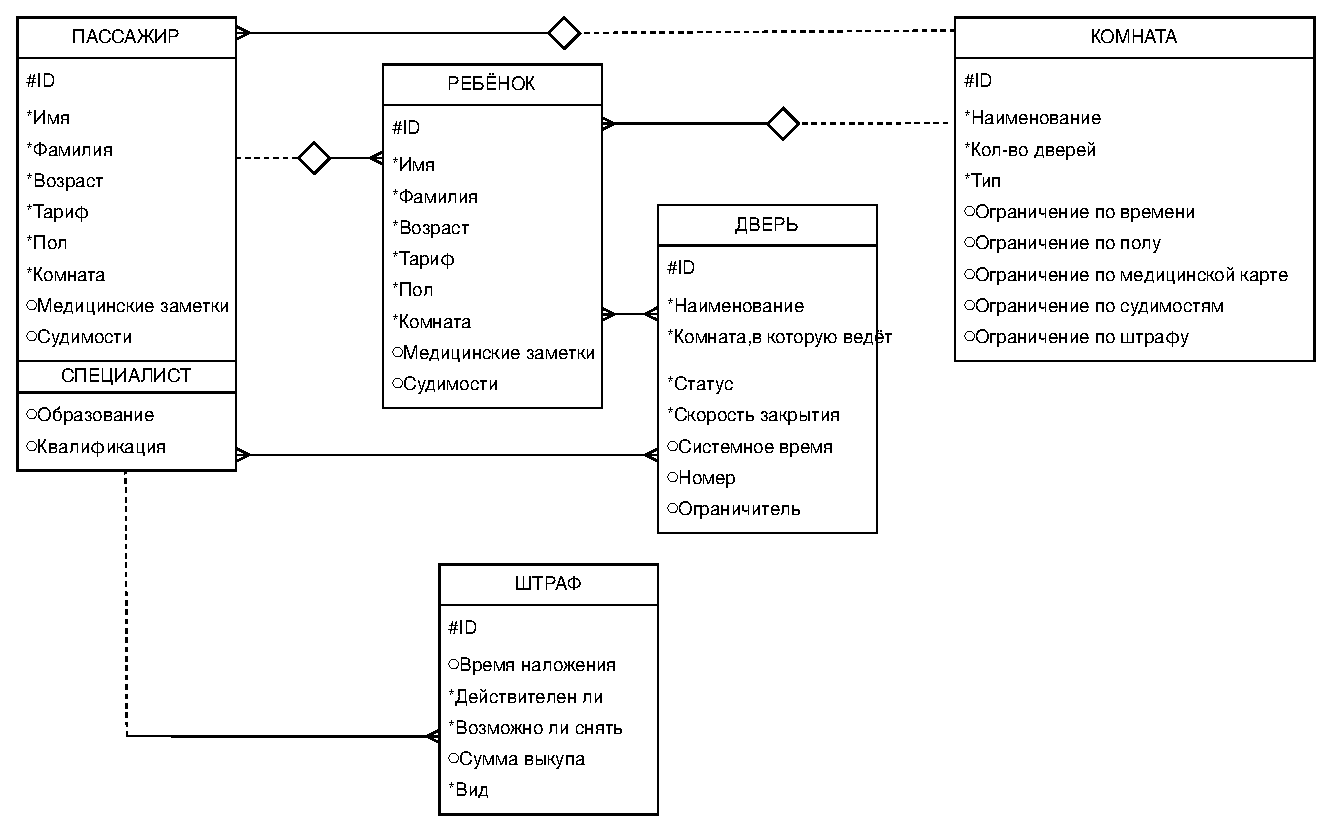
\includegraphics[width=1\linewidth]{images/ER}
	\caption{ER- диаграмма}
	\label{fig:er}
\end{figure}

\subsubsection{Архитектура системы}

Приложение разработано на языке Python с использованием библиотеки tkinter. Через библиотеку sqlite3 программа взаимодействует с СУБД SQLite.

\subsubsection{Функциональные требования к программной системе}

На основании анализа предметной области, разрабатываемая программная система «СКУД на круизном лайнере» должна включать в себя следующие ключевые функциональные возможности:
\begin{itemize}
	\item Открыть/закрыть таблицу
	\item Редактировать таблицу
	\item Перейти к следующему/предыдущему элементу
	\item Добавить новый элемент -- Реализация опции добавления нового элемента с последующей актуализацией этих данных в БД 
	\item Редактировать выбранный элемент -- Реализация опции редактирования элемента с последующей актуализацией этих данных в БД 
	\item Найти элемент по идентификатору
	\item Удалить элемент -- Реализация опции редактирования элемента с последующей актуализацией этих данных в БД 
\end{itemize}

\subsubsection{Моделирование вариантов использования}

На рисунке  ~\ref{fig:commonscheme2} представлена диаграмма прецедентов, которая служит важным средством для систематизации функциональных требований и возможностей системы, выявляя ключевые сценарии использования. Диаграмма прецедентов изображает, как пользователи могут взаимодействовать с системой, а также помогает выявить набор основных функциональных возможностей, доступных пользователям.

При построении диаграммы вариантов использования применяется унифицированный язык визуального моделирования UML.

Каждый прецедент на диаграмме отражает отдельный путь взаимодействия в системе и представляет потенциальные действия, которые могут быть предприняты пользователями в различных ролях. Пользователем или действующим лицом является сущность, взаимодействующая с системой извне (например, человек, техническое устройство).

\begin{figure}
	\centering
	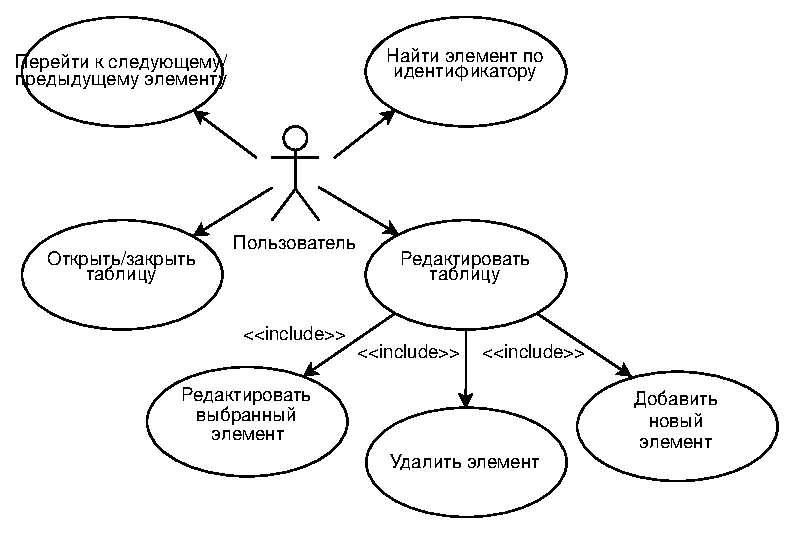
\includegraphics[width=1\linewidth]{images/CommonScheme2}
	\caption{Диаграмма прецедентов}
	\label{fig:commonscheme2}
\end{figure}

\subsubsection{Вариант использования <<Открыть/закрыть таблицу>>}

Пользователь выбирает интересующую его таблицу из списка предложенных и открывает окно, репрезентирующее требуемый от приложения интерфейс.

\subsubsection{Вариант использования <<Редактировать таблицу>>}

Пользователь решает внести какие-либо изменения в таблице. Он может сделать это, добавляя новые элементы, удаляя или редактируя существующие.

\subsubsection{Вариант использования <<Перейти к следующему/предыдущему элементу>>}

Пользователь листает элементы в таблице посредством перехода к предыдущему/следующему за текущим.

\subsubsection{Вариант использования <<Найти элемент по идентификатору>>}

Пользователь решает не листать элементы по одиночке т.к. не хочет тратить на это время. Он помнит идентификатор искомого элемента, вводит его в предназначенное текстовое поле и переходит к искомому элементу.

\subsubsection{Вариант использования <<Добавить новый элемент>>}

Пользователь заполняет поля данных будущего объекта и добавляет его в таблицу по клику.

\subsubsection{Вариант использования <<Редактировать выбранный элемент>>}

Пользователь редактирует необходимые ему поля у текущего элемента и вносит эти изменения в таблицу по клику.

\subsubsection{Вариант использования <<Удалить элемент>>}

Пользователю больше не нужен выбранный элемент и он стирает его в таблице по клику.

\subsection {Нефункциональные требования к программной системе}
\subsubsection{Требования к надежности}
Для обеспечения надёжной работы базы данных, она должна быть приведена в нормализированный по трём формам вид:
-Первая нормальная форма (1NF)

Все атрибуты объекта ПАССАЖИР имеют только одно значение.

Все атрибуты объекта РЕБЁНОК имеют только одно значение.

Все атрибуты объекта ДВЕРЬ имеют только одно значение.

Все атрибуты объекта КОМНАТА имеют только одно значение.

Все атрибуты объекта ШТРАФ имеют только одно значение.

Все атрибуты объекта пересечения ДОСТУПЫ имеют только одно значение.

Все атрибуты объекта пересечения ДОСТУПЫ ЧС имеют только одно значение.


-Вторая нормальная форма (2NF)

Атрибуты объекта ПАССАЖИР зависят от полного UID (id пассажира).

Атрибуты объекта РЕБЁНОК зависят от полного UID (id ребёнка).

Атрибуты объекта ДВЕРЬ зависят от полного UID (id двери).

Атрибуты объекта КОМНАТА зависят от полного UID (id Комнаты).

Атрибуты объекта ШТРАФ зависят от полного UID (id штрафа).

Атрибуты объекта пересечения ДОСТУПЫ зависят от двойного UID.

Атрибуты объекта пересечения ДОСТУПЫ ЧС зависят от двойного UID.


-Третья нормальная форма (3NF)
При проверке всех объектов не было выявлено независимых от UID атрибутов или атрибутов, зависимых от других атрибутов.

На основе ER-модели данных построена реляционная модель данных, которой должна соответствовать БД. Она показанная на рисунке  ~\ref{fig:commonscheme3}

\begin{figure}
	\centering
	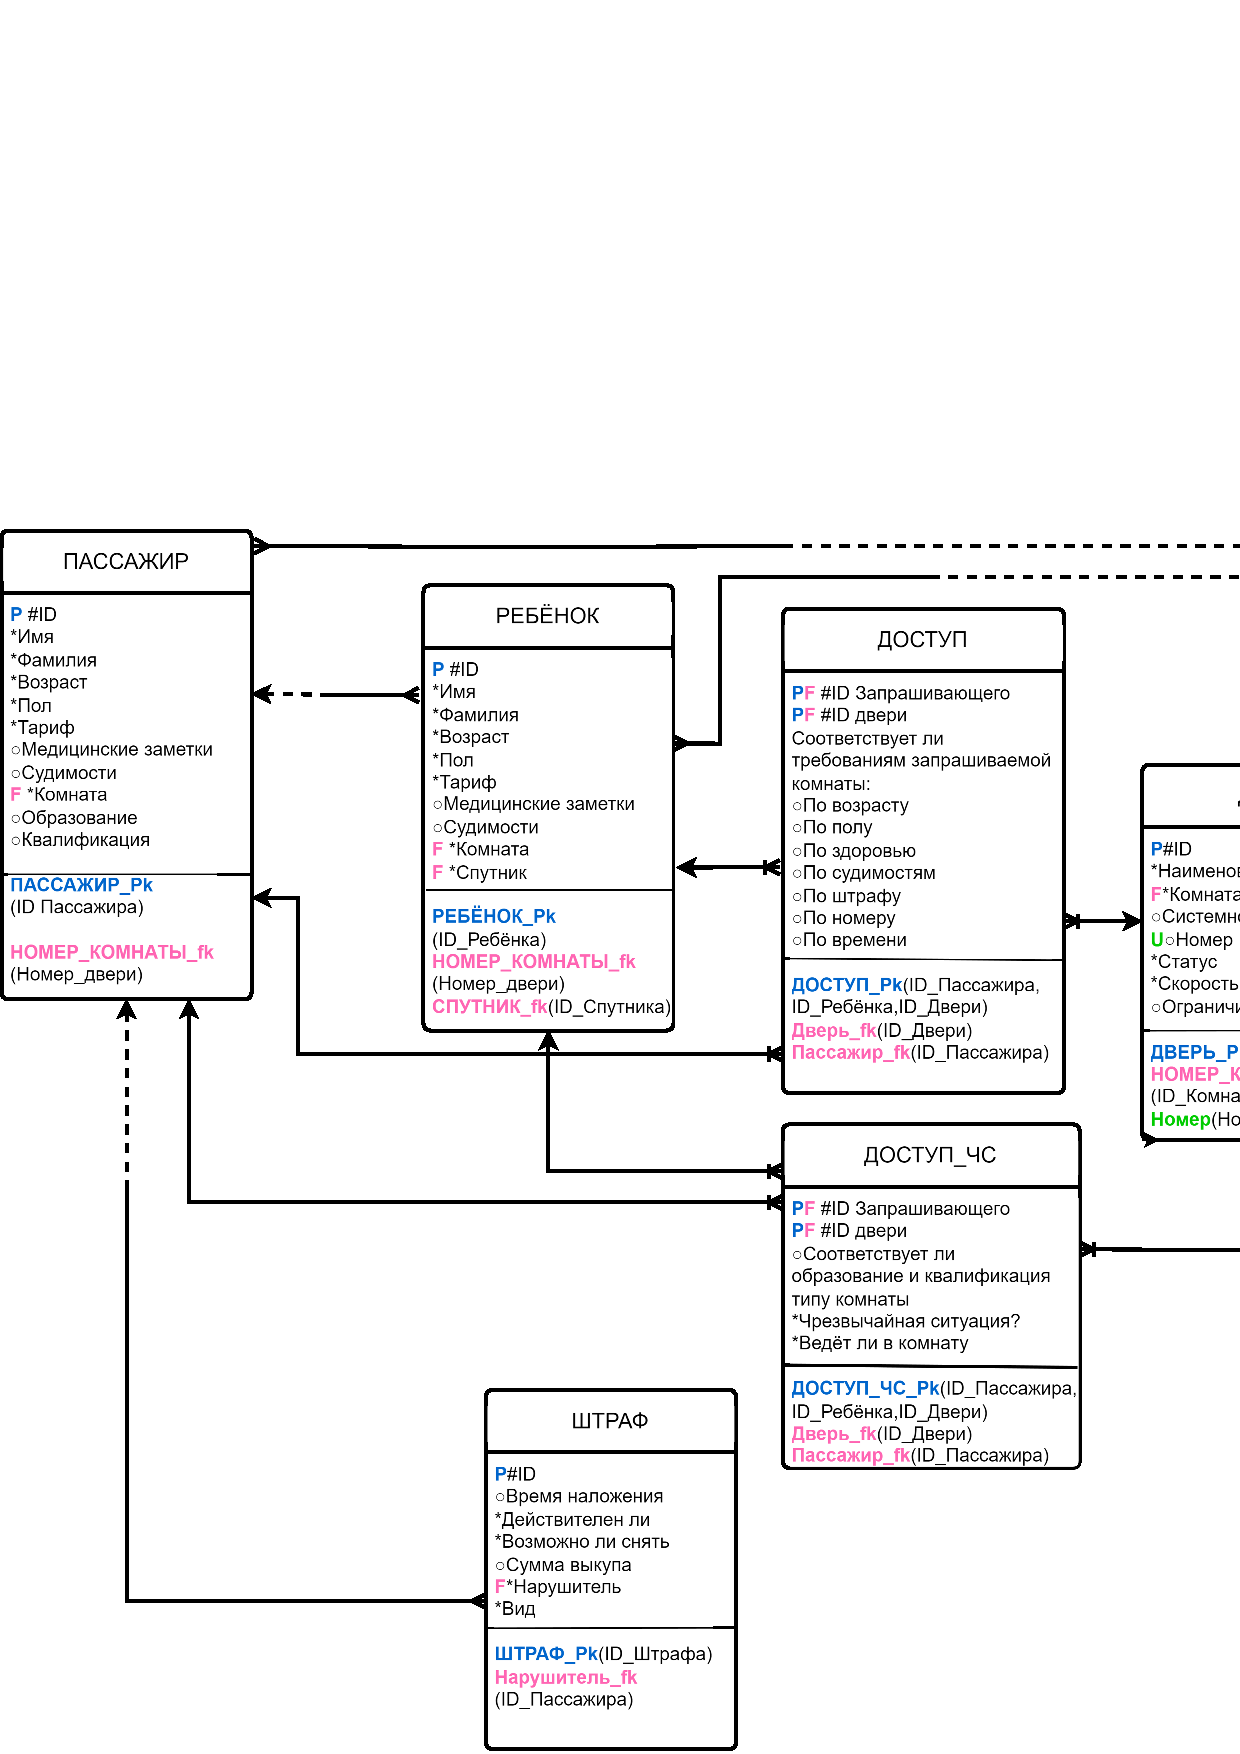
\includegraphics[width=1\linewidth]{images/CommonScheme3}
	\caption{Реляционная модель данных}
	\label{fig:commonscheme3}
\end{figure}

\subsubsection{Требования к безопасности}
1. Поддержка современных операционных систем, обеспечивающая стабильную и безопасную работу на различных платформах;

2. Реализация защиты от атак типа SQL-инъекций, предотвращающая нежелательное вмешательство в работу приложения;

3. Регулярное обновление компонентов системы для предотвращения уязвимостей, связанных с устаревшим программным обеспечением.

\subsubsection{Требования к программному обеспечению}
Для реализации программной системы должны быть использованы следующие языки программирования: 

Python - основной язык реализации приложения; 

SQL - язык структурированных запросов к базе данных.

Для работы и приложения требуется ОС Windows 7 или более поздняя версия/Ubuntu 16.0 или более поздняя версия с установленным интерпретатором языка python и установленной СУБД SQLite.

\subsubsection{Требования к аппаратному обеспечению}
Системе необходим центральный процессор с количеством ядер от 2 и выше с частотой ядра от 1.4 ГГц. Объем оперативной памяти – 4 Гб.
Свободное место на диске: 13МБ

\subsection{Требования к оформлению документации}

Требования к стадиям разработки программ и программной документации для вычислительных машин, комплексов и систем независимо от их
назначения и области применения, этапам и содержанию работ устанавливаются ГОСТ 19.102–77. Программная документация должна включать в себя:

1. Анализ предметной области;

2. Техническое задание;

3. Технический проект;

4. Рабочий проект.

